% !TEX encoding = UTF-8 Unicode
% Modelo para livros da coleção "As grandes ideias de todos os tempos" (Globo Livros)
% Compilar com pdflatex (duas vezes para referências internas)

\documentclass[12pt, openany]{book} % openany para capítulos começarem em qualquer página (opcional)

% =================== PACOTES ===================
\usepackage[utf8]{inputenc}
\usepackage[T1]{fontenc}
\usepackage[brazil]{babel}      % hifenização e termos em português
\usepackage{graphicx}            % figuras
\usepackage{xcolor}               % cores
\usepackage{geometry}             % margens
\usepackage{fancyhdr}             % cabeçalhos/rodapés
\usepackage{titlesec}             % formatação de títulos
\usepackage{tcolorbox}            % caixas coloridas
\tcbuselibrary{skins, breakable}
\usepackage{marginnote}           % notas marginais
\usepackage{caption}              % legendas
\usepackage{hyperref}             % links (opcional, mas recomendado)
\usepackage{blindtext}            % texto de exemplo (remover no documento real)

% =================== CONFIGURAÇÕES ===================
% --- Margens ---
\geometry{
  a4paper,
  top=2.5cm,
  bottom=2.5cm,
  inner=2.5cm,
  outer=2.5cm,
  marginparwidth=2cm,
  marginparsep=5mm
}

% --- Cores da coleção (exemplo: azul escuro e laranja) ---
\definecolor{corprincipal}{RGB}{0, 51, 102}      % azul escuro
\definecolor{corsecundaria}{RGB}{255, 140, 0}    % laranja
\definecolor{corfundo}{RGB}{245, 245, 245}       % cinza claro para fundos

% --- Estilo de páginas ---
\pagestyle{fancy}
\fancyhf{}
\fancyhead[LE,RO]{\thepage}
\fancyhead[RE]{\nouppercase{\leftmark}}   % título do capítulo à direita nas páginas pares
\fancyhead[LO]{\nouppercase{\rightmark}}  % título da seção à esquerda nas páginas ímpares
\renewcommand{\headrulewidth}{0.5pt}
\renewcommand{\footrulewidth}{0pt}

% --- Estilo de capítulo ---
\titleformat{\chapter}[display]
  {\normalfont\Huge\bfseries\color{corprincipal}}
  {\filleft\Large\color{corsecundaria} Capítulo \thechapter}
  {1ex}
  {\titlerule\vspace{1ex}\filright}
  [\vspace{1ex}\titlerule]

% --- Estilo de seção ---
\titleformat{\section}
  {\normalfont\Large\bfseries\color{corprincipal}}
  {\thesection}{1em}{}

% --- Estilo de subseção ---
\titleformat{\subsection}
  {\normalfont\large\bfseries\color{corprincipal!80!black}}
  {\thesubsection}{1em}{}

% =================== AMBIENTES PERSONALIZADOS ===================
% Caixa para "Ideia central"
\newtcolorbox{ideia}[1][]{
  colback=corfundo,
  colframe=corprincipal,
  fonttitle=\bfseries,
  title=Ideia central,
  sharp corners,
  boxrule=0.5mm,
  left=2mm,
  right=2mm,
  top=2mm,
  bottom=2mm,
  #1
}

% Caixa para biografia
\newtcolorbox{biografia}[1][]{
  colback=corfundo,
  colframe=corsecundaria,
  fonttitle=\bfseries,
  title=Biografia,
  sharp corners,
  boxrule=0.5mm,
  left=2mm,
  right=2mm,
  top=2mm,
  bottom=2mm,
  #1
}

% Caixa para linha do tempo
\newtcolorbox{linhadotempo}[1][]{
  colback=white,
  colframe=corprincipal,
  colbacktitle=corprincipal!20,
  fonttitle=\bfseries,
  title=Linha do tempo,
  sharp corners,
  boxrule=0.5mm,
  left=2mm,
  right=2mm,
  top=2mm,
  bottom=2mm,
  #1
}

% Comando para nota marginal destacada
\newcommand{\conceito}[1]{\marginnote{\small\bfseries\color{corsecundaria} #1}}

% =================== INÍCIO DO DOCUMENTO ===================
\begin{document}

% --- Página de rosto (exemplo) ---
\begin{titlepage}
  \centering
  \vspace*{1cm}
  {\Huge\bfseries\color{corprincipal} O Livro da Filosofia\par}
  \vspace{1.5cm}
  {\Large As grandes ideias de todos os tempos\par}
  \vspace{2cm}
  {\large Globo Livros\par}
  \vfill
  {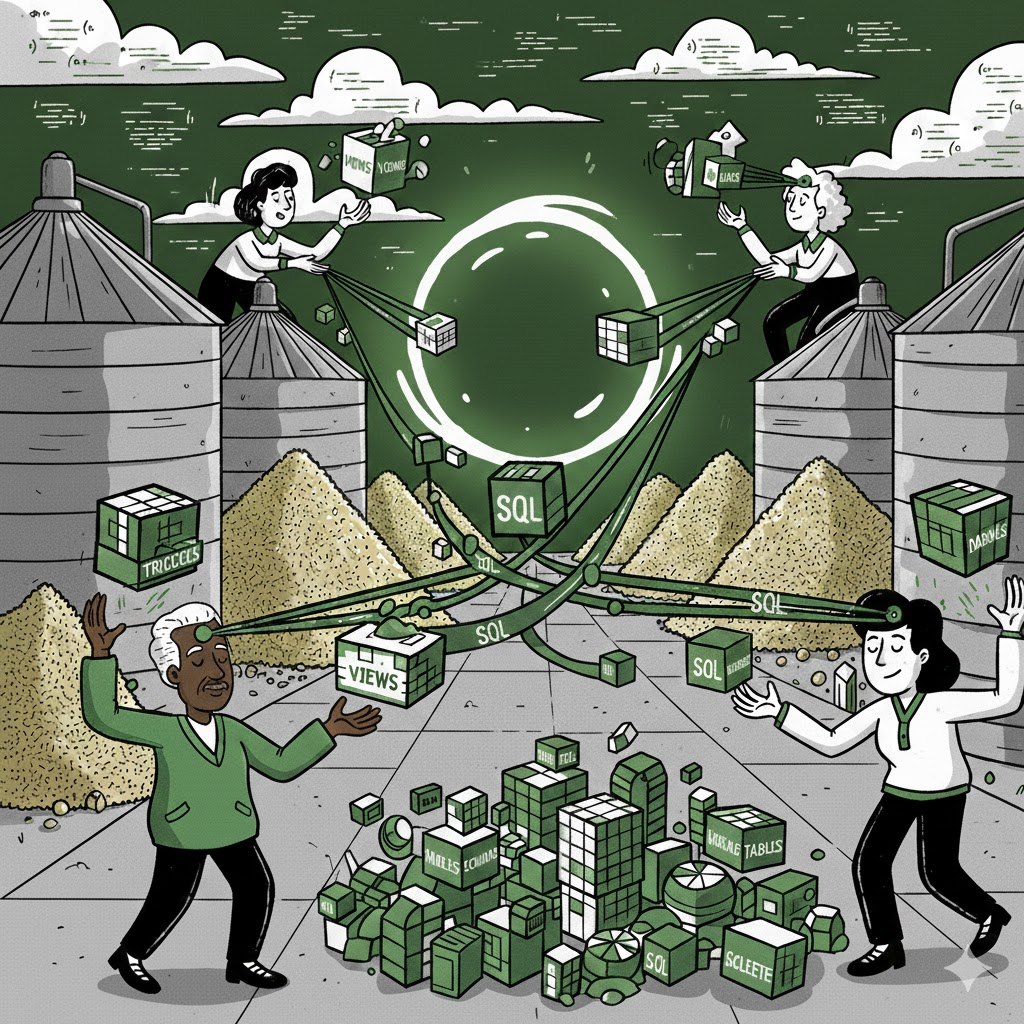
\includegraphics[width=0.3\textwidth]{capa.jpg}\par} % substitua pelo arquivo de capa
  \vfill
\end{titlepage}

% --- Sumário ---
\tableofcontents
\thispagestyle{empty}
\clearpage

% --- CAPÍTULO EXEMPLO ---
\chapter{O que é a verdade?}

\conceito{Verdade como correspondência}
Neste capítulo exploramos as principais teorias da verdade ao longo da história.

\section{Teoria da correspondência}
\blindtext

\begin{ideia}
  \textbf{Correspondência:} uma proposição é verdadeira se corresponde aos fatos. Essa visão remonta a Aristóteles.
\end{ideia}

\subsection{Origem em Aristóteles}
\blindtext

\begin{biografia}
  \textbf{Aristóteles} (384–322 a.C.) – filósofo grego, discípulo de Platão, autor da \emph{Metafísica} e da \emph{Ética a Nicômaco}.
\end{biografia}

\section{Teoria da coerência}
\blindtext

\begin{linhadotempo}
  \begin{itemize}
    \item[1920] Desenvolvimento do positivismo lógico
    \item[1930] Publicação de \emph{A Lógica da Descoberta Científica} (Popper)
    \item[1950] Debate entre correspondência e coerência
  \end{itemize}
\end{linhadotempo}

\subsection{Influências no século XX}
A teoria da coerência ganhou força com os filósofos idealistas, como Bradley, e posteriormente foi retomada por Neurath e Hempel.

% --- Figura de exemplo ---
\begin{figure}[htbp]
  \centering
  
\includegraphics[width=0.6\textwidth]{Universidade_de_Rio_Verde.jpg} % substitua pelo arquivo de figura
  \caption{Representação esquemática da teoria da correspondência.}
  \label{fig:correspondencia}
\end{figure}

A Figura~\ref{fig:correspondencia} ilustra a relação entre linguagem e mundo.

\section*{Para saber mais}
Algumas leituras recomendadas:
\begin{itemize}
  \item \emph{Investigações Filosóficas}, L. Wittgenstein
  \item \emph{Verdade e Método}, H.-G. Gadamer
\end{itemize}

% --- FIM DO DOCUMENTO ---
\end{document}